\section{Decision Tree}

Constructing a decision tree is a good way to see first correlations.

To get a decision tree from a dataset different ways are possible. We are concentrating on the simple information gain and applying again RapidMiner on the dataset. 

\subsection*{RapidMiner and decisiontrees}
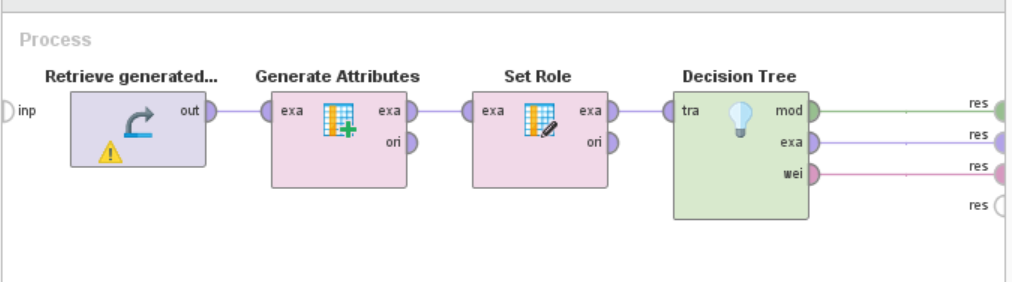
\includegraphics[width = 0.9\textwidth]{DecisionTreeRapidModel.PNG}

RapidMiner does the following steps:
\begin{description}
	\item[Retrieve] Includes the dataset
	\item[Generate Attribute] Changes the Numerical Attribute strata to a nominal one
	\item[Set Role] Gives strata the label role, so that the decision tree ends with this
	\item[Decision Tree] Creates a decision tree
\end{description}

Furthermore we choose information gain as splitting criterium (minimal gain 0.1) and a confidence of 0.25.

\subsection*{Full dataset}

Applying this process on the full dataset we get the not really helpful tree:

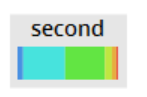
\includegraphics[width=0.9\textwidth]{DecisionTreeRapidTreeFull.PNG}



%13 für vector 200
